The matrix has been defined in the "Q0038.py", and probably has some typo errors due to having to enter it by hand. It has been defined in the code as thus:\\
\begin{figure}[ht]
  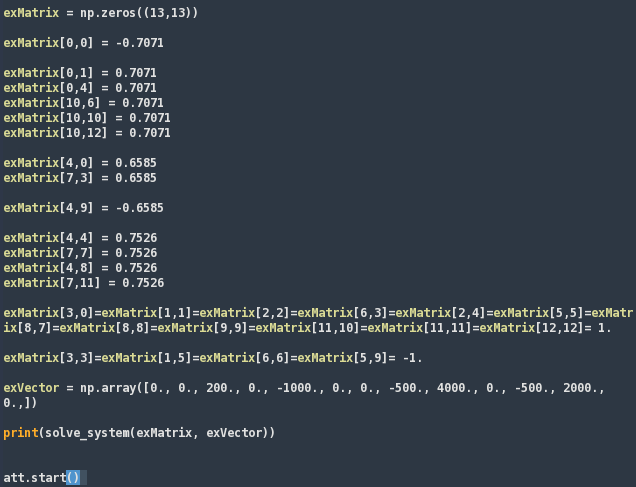
\includegraphics[width=1\linewidth]{linear_system}
  \caption{The linear system of equations being entered into a matrix}
\end{figure}

Passing this matrix into the \textit{solve\_system} function returns the following vector as the solution:
$$
\begin{pmatrix}
  -2320.09555208 \\
  0. \\
  2520.09555208 \\
  -2320.09555208 \\
  -2320.09555208 \\
  0. \\
  -2320.09555208 \\
  978.62498865 \\
  3021.37501135 \\
  0. \\
  1612.98198965 \\
  387.01801035 \\
  0.
\end{pmatrix}
$$
